To evaluate our proposed module system we carried out a case study where
the JastAdd Extensible Java Compiler (JastAddJ), a system entirely based on
inter-type declarations, was retrofitted to use modules. JastAddJ is a
modular Java compiler designed particularly with extensibility in mind,
that uses ITDs and attribute grammars as its main modularisation
mechanisms.  We have previously reported on the merits of this combination
in \cite{aosd08abc}. However, there are some nuicenses related to using
multiple variants in the same system and certain properties with
unnecessary global scope that makes it a prime target for our proposed
module system. 

We believe this application serves as a suitable case to study when
evaluating the merits of the module system on realistic examples for
several reasons: 1) It is a reasonably sized application of more than
21.000 lines of code not counting documentation and white space.  3) It is
designed using ITDs from the beginning, completely separating behaviour
from the class hierarchy using the paradigm that "everything is an ITD". 2)
The system is commonly used in various applications requiring extensible
compiler frontends, e.g., the Soot bytecode manipulation framework, and the
AspectBench Compiler.

\subsection{JastAdd Java Compiler Overview}
\label{jastaddjoverview}
The compiler consists of four main components: a \emph{Java 1.4 frontend}
with a corresponding \emph{Bytecode backend}, a \emph{Java 5 frontend} with
a \emph{Bytecode backend} as illustrated by Figure~\ref{MainComponents}. 

\begin{figure}[htb!]
  \begin{center}
    \resizebox{8.5cm}{!}{
      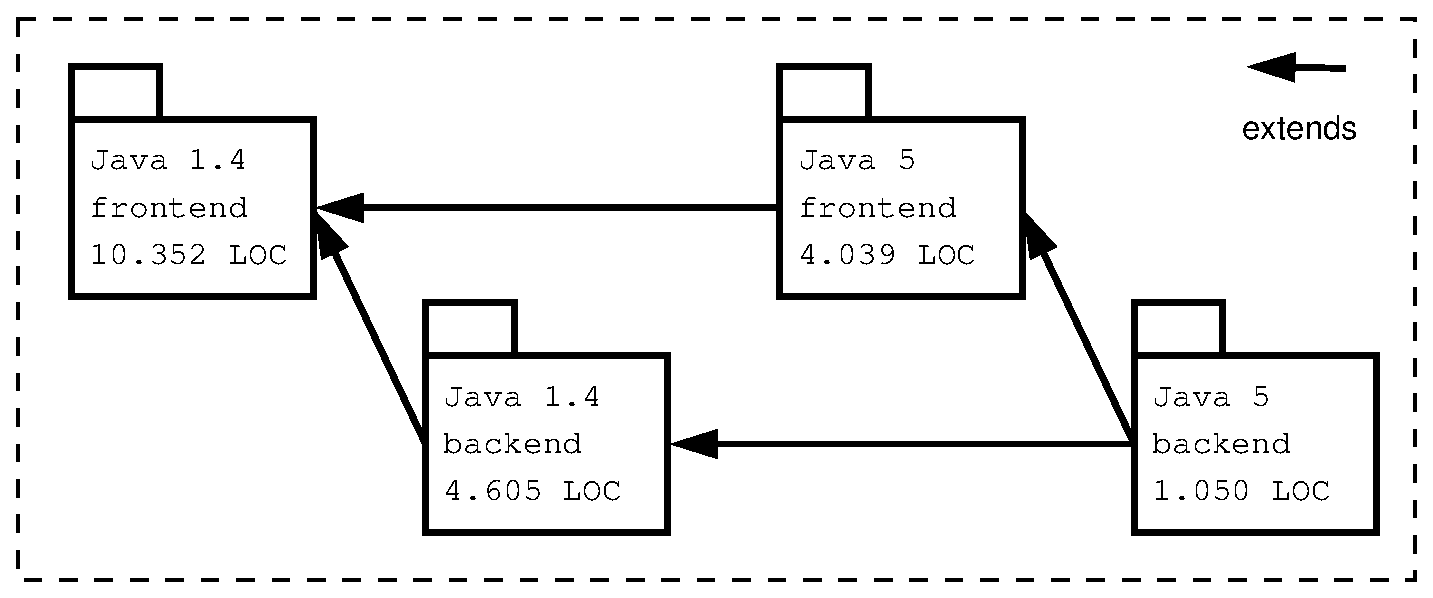
\includegraphics{figures/MainComponents}
    }
    \caption{The main components of JastAddJ}
    \label{MainComponents}
  \end{center}
\end{figure}

Since there is no module system each component is represented as a
directory of reusable source files that are combined using build files. The
Java 5 frontend is an extension to the Java 1.4 frontend, reusing its
source file, while specifying Java 5 language features as an increment to
the Java 1.4 frontend. A build file to create a Java 1.4 semantic checker
will thus only include files from the Java 1.4 folder, while a build file
for a Java 5 semantic checker includes files from both folders. The
backends are extensions to the frontends and reuse source files in a
similar manner.  By changing which files to include in the build it is
possible to build four different tools from these components.

Each frontend can be further divided into the following subcomponents: a
parser that builds an AST, a bytecode reader that reads class files, and a
semantic analyzer or code generator. The parser is generated from a context
free grammar, the bytecode reader is written in plain Java, and the
analyzers and code generators are implemented using attribute grammars and
inter-type declarations.

The architecture has a few problems that can be elegantly solved using a
module system. First, the different variants of the compiler can not
coexist in the same system since ITDs destructively update the class
hierarchy. This is handled with an ugly hack where multiple build files and
scripts are used generate compilers to different packages.  Second, the
bytecode readers are implemented in plain Java in a fashion which
unfortunately makes them quite hard to extend and we therefore use
different implementations of the reader in the Java 1.4 frontend and the
Java 5 frontend. This is handled by including different versions of source
files in the build for the Java 5 frontend and excluding some of the files
in the Java 1.4 frontend. Third, the systems are composed into one global
namespace which is terrible from an information hiding point of view.

\subsection{Applying Modules}

Imports, merge (to share frontend types)

changes:
split ast and jrag
permissions

new diagram

a few code snippets

\subsection{Evaluation}

Shows dependencies explicitly, information hiding, enables sharing through merge

everything used to be globally visible
  modules improves information hiding 
    (concrete example would be nice)
    percent that became non-global

enables variants with different sets of ITDs
  examples
enables variants with replaced/overridden classes
  example: bytecode reader
  (reason, monolithic implementation not suitable for extension, therefore
  replacement easier)

can we characterize the typical changes needed?
how intrusive/global were the changes?

eliminate cycles as a side-effect
  required by the module system
  architecture improved/ should have been done that way from the beginning
  in retrospect



many properties
are global even though a more local scope would improve information hiding.

improve extensibility and information hiding



 
 
